\documentclass{article}
\usepackage{microtype,graphicx,booktabs,amsmath,amssymb,amsthm,hyperref}
\usepackage[preprint]{icml2026}
\newtheorem{proposition}{Proposition}
\newtheorem{theorem}{Theorem}
\newcommand{\R}{\mathbb R}
\newcommand{\E}{\mathbb E}
\newcommand{\norm}[1]{\left\|#1\right\|}
\newcommand{\ip}[2]{\langle #1,#2\rangle}
\newcommand{\Haar}{\mathsf H}
\icmltitlerunning{Auditing Population Uncertainty in Cryo-EM}
\begin{document}
\twocolumn[
\icmltitle{Auditing Population Uncertainty in Cryo-EM:\\Numerical Integration, Nuisance Laws, and Identifiability}
\begin{icmlauthorlist}\icmlauthor{Fourier Cryo Splats Project}{anon}\end{icmlauthorlist}
\icmlaffiliation{anon}{Fourier Cryo Splats research project}
\icmlcorrespondingauthor{Project repository}{\url{https://github.com/yashpatel5400/fourier-cryo-splats}}
\icmlkeywords{cryo-EM, uncertainty quantification, Gaussian representations, population inference}
\vskip .2in]
\printAffiliationsAndNotice{}
\hypersetup{pdftitle={Auditing Population Uncertainty in Cryo-EM: Numerical Integration, Nuisance Laws, and Identifiability}}
\begin{center}\small Development manuscript; not submitted.\end{center}

\begin{abstract}
A detailed cryo-electron microscopy reconstruction does not by itself support
calibrated uncertainty about density or conformational populations. Starting
from conjugate-paired Fourier Gaussian reconstructions of three experimental
stacks, we examine whether population inference is a defensible next target.
Matched simulations separate information discarded by moment summaries from
numerical error in orientation marginalization. Fixed template-bank statistics
have 29--55 times the squared separation of the best tested moment contrasts,
but are inaccurate marginal likelihood approximations. One continuous
importance-sampling repair passes an unchanged numerical gate on all three
stacks. A simulation-only posterior-draw diagnostic shows why agreement
between banks still cannot certify absolute integrals. We derive the implicit
known-pose population bias caused by state-dependent viewing laws and show
that bounded scores cannot be exactly unbiased over arbitrary continuous
state-specific amplitude intervals. A frozen materiality screen then fails
on all three compact-region targets: maximum modeled population biases are
.000214, .000122 and .003493, below .02. These results end that proposed method
branch. Recorded acquisition metadata and corner spectra expose further gaps
between the simulator and experimental inference. We provide reproducible
diagnostics and explicit limitations, not a validated population-uncertainty
method or a claim of experimentally calibrated coverage.
\end{abstract}

\section{Introduction}
Cryo-EM reconstruction combines noisy two-dimensional projections, uncertain
orientations and imaging parameters, and potentially heterogeneous molecular
states. Neural implicit fields and Gaussian representations can recover
complex structures, but representation quality and uncertainty calibration
are different properties. Fourier shell correlation (FSC), posterior
dispersion, independent-particle prediction and coverage of a population
fraction answer different questions. An uncertainty study must specify its
target before selecting a baseline or interpreting agreement.

Our project began with Gaussian kernels in Fourier space and subsequently
studied confidence intervals for fixed density features. The resulting
pose-aware intervals were uninformative in the tested end-to-end simulator;
moment-based candidate tests were sensitive to uncalibrated viewing and noise
assumptions. Rather than adding another interval to that construction, this
manuscript asks a narrower question: \emph{do the available data and numerical
tools justify developing population uncertainty for two nominated structures?}
The answer for the compact perturbations tested here is no.

This conclusion requires distinguishing three obstacles. A summary statistic
may discard information even when its moments are computed exactly. A richer
likelihood statistic may retain discrimination while failing as a numerical
marginal likelihood. Finally, a proposed nuisance-robust population method
may address an effect too small to motivate that method on its nominated
targets. Improving the second obstacle does not resolve the third.

We contribute an auditable investigation of these obstacles, with fixed
computational and scientific stopping rules. The numerical repair is classical
importance sampling, not a new inference principle. The population-score
identity and amplitude obstruction are elementary results with explicit
scope; we do not claim priority for general mixture or analytic-continuation
arguments. The empirical contribution is the matched three-stack diagnosis
and its unfavorable decision, supported by saved arrays and independent
calculations. An experimentally useful uncertainty method, a demonstrated
advantage over matched population baselines, and submission-level novelty
remain unresolved.

\section{Targets and Closest Prior Work}
\label{sec:prior}
\paragraph{Reconstruction and density uncertainty.}
Bayesian cryo-EM reconstruction is established \citep{scheres2012}.
Gaussian pseudo-atom posterior inference \citep{joubert2015}, variational
Fourier-slice uncertainty \citep{ullrich2020}, and joint likelihood-Hessian
analysis \citep{rangan2024} precede the present work. CryoDRGN and
CryoDRGN-AI address heterogeneous representation learning and ab initio
reconstruction \citep{zhong2021,drgnai2025}; a fixed-pose homogeneous fit
does not reproduce their full tasks. Gaussian representations are likewise
not new to cryo-EM \citep{chen2021,chen2025,qu2025,shekar2025}.

\paragraph{Populations and likelihoods.}
BioEM marginalizes image nuisances and evaluates candidate structures
\citep{bioem2013}; CryoLike supplies modern likelihood tooling
\citep{cryolike2025}. Cryo-BIFE already samples population/free-energy
uncertainty along a nominated conformational path, using BioEM nuisance
integration \citep{cryobife2021}. RECOVAR accounts for noisy latent
coordinates in heterogeneity and population estimation \citep{recovar2025}.
Whole-stack ensemble reweighting can correct severe distortions from hard
or soft particle counting \citep{counting2026}. Thus posterior sampling or
a two-state likelihood alone is not a contribution. The uncertainty target
here would be a population \emph{among selected particles}, not an equilibrium
solution population unaffected by acquisition and selection.

\paragraph{Viewing laws and numerical marginalization.}
Nonuniform views matter in moment recovery \citep{sharon2020,subspacemom2026},
structural comparison \citep{momentmetrics2024}, and misspecified likelihood
\citep{nonuniformmle2025}. The recent Bayesian orientation discussion
explicitly considers estimating the view prior jointly with structure
\citep{bayespose2026}. Adaptive proposals, smoothing and a uniform defensive
component were already used for cryo-EM marginalization by
\citet{brubaker2015}. Our continuous quaternion proposal is numerical repair
within that tradition. Agreement of independent approximations is weaker
than a certificate of the integral; posterior-draw diagnostics for simulated
data are also established \citep{grosse2015}.

\paragraph{Validation and the calibration unit.}
Gold-standard halves and noise substitution address reconstruction overfitting
\citep{schereschen2012,chen2013}; confidence maps address signal significance
\citep{beckers2019,beckers2020}; independent-particle tests assess image fit
\citep{independent2020}. None is automatically a confidence interval for a
biological population. CryoBench and CAHRA separate volume, latent-state,
population and pose tasks \citep{cryobench2025,cahra2026}. The broader survey
in Appendix~\ref{app:survey-new} documents related uncertainty targets and
reading limits. Its 141 candidates are not 141 fully audited methods.

\section{Forward Model and Gaussian Reconstructions}
For $F(k)=\int\rho(x)e^{-2\pi i k^\top x}\,dx$, the observation model is
\begin{equation}\label{eq:forward-new}
 Y_i(q)=a_i C_i(q)e^{-2\pi i q^\top t_i}F_{Z_i}(E_iq)+\epsilon_i(q).
\end{equation}
$Z_i$ is molecular state, $E_i$ the oriented central plane, $t_i$ shift,
$C_i$ CTF and $a_i$ real amplitude. Population inference must specify which
of these are observed, marginalized or uncertain. Throughout our new
numerical diagnostics, templates, one CTF and zero shifts are fixed;
orientations are Haar and each realified Fourier-noise coordinate is
independent $N(0,1)$. These are simulator assumptions, not measurements of
experimental nuisance distributions.

Our original reconstruction parameterization uses paired spectral kernels:
\begin{align}\label{eq:splats-new}
F_\theta(k)&=\sum_j\{c_j G_j(k-\mu_j)+\overline c_jG_j(k+\mu_j)\},\\
G_j(u)&=\exp(-u^\top\Lambda_j u/2),\quad \Lambda_j\succ0.\nonumber
\end{align}
Real precision matrices and conjugate pairing enforce
$F_\theta(-k)=\overline{F_\theta(k)}$; self-conjugate terms are real.
The dense differentiable reference allows movable centers and anisotropic
precisions. The \emph{actual three-stack benchmark} fits a sparse fixed
lattice and isotropic width, with real/imaginary coefficients tied across
conjugate nodes. It does not demonstrate adaptive anisotropic splatting.
Tomographic projection is linear Fourier slicing, without optical alpha
compositing.

The new diagnostics use the saved $64^3$ fitted maps as constant-cell
templates with exact cell Fourier factors, evaluated by NUFFT and selected
independent direct sums. This makes off-grid orientation evaluation explicit;
it does not preserve an unrestricted spectral representation or eliminate
template error. Each map is normalized to unit array $L^2$ norm. A previously
fixed Gaussian mask of width 20\,\AA\ is centered at its largest smoothed
peak in the central half-field cube. Write $\rho_G=\rho M$ and
$\rho_\delta=\rho-\delta\rho_G$. These are artificial local perturbations,
not experimentally labeled conformations or measured biochemical occupancy.

\section{Numerical and Statistical Diagnostics}
\subsection{Information retained by a fixed statistic}
For a scalar score $T$, define
\begin{equation}\label{eq:separation-new}
D(T)=\frac{(\E_1T-\E_0T)^2}{\operatorname{Var}_0(T)}.
\end{equation}
We compare power and power-plus-bispectrum contrasts, including separately
trained classical covariance-aware directions, with a frozen template-bank
log ratio. All use the same candidate, region, transfer, 220 frequencies and
8,192 paired noise/view draws. We retain both 32,768-point banks, four
quadrature prefixes and all four nonzero deletion fractions.

A finite-bank log ratio remains a statistic if its quadrature is poor.
Its measured $D$ is therefore a descriptive separation, but it is not the
KL divergence of the continuous image model or an information ceiling.
We estimate the gap SE with the paired draws and the SE of $D$ with a
delta calculation that also includes variance-estimation uncertainty
(Appendix~\ref{app:stats-new}). No normal power guarantee is inferred.

\subsection{A fixed orientation-integration repair}
For a fixed image and map, integrate the positive Gaussian residual kernel
$f_y(R)$ over normalized Haar measure, with integral $I_y$.
For independent $R_l\sim q_y$,
\begin{equation}
 \widehat I_y=\frac1L\sum_{l=1}^L f_y(R_l)/q_y(R_l).
\end{equation}
The omitted Gaussian normalization is common to the compared maps.
The proposal is fit using the image and the midpoint template, then frozen
before either importance bank. Attempt one combines eight locally optimized
angular central Gaussian (ACG) quaternion components with .05 Haar mass.
It fails the declared gate on two stacks.

The one permitted repair reuses all local fits and assigns masses .45 to
the local mixture, .50 to a catalogue mixture and .05 to Haar. Catalogue
centers are the same 32,768 training rotations; weights are proportional to
the midpoint likelihood raised to $1/2$. Every center receives an isotropic
ACG kernel with an 8-degree scale parameter, not an 8-degree angular
standard deviation. Continuous rotations are sampled from this mixture,
and its \emph{full} density is evaluated using all centers. There is no
top-$k$ replacement of the target integral. Appendix~\ref{app:numerics-new}
gives the density and all fixed choices.

Both attempts use the same 64 source indices, two generating states and
two 8,192-draw banks per stack. A stack passes if at least 90\% of its 128
images have bank log-ratio discrepancy at most .01, and all four median
importance ESS values exceed 256. All three must pass. This is a necessary
feasibility gate, not a sufficient numerical or inferential certificate.

\subsection{Simulation-only posterior-draw check}
The generating pose of a correctly simulated image is a posterior draw
conditional on that image. This premise can expose a common missed mode
even when two ordinary banks agree \citep{grosse2015}.

\begin{proposition}[Reciprocal identity]\label{prop:planted-new}
Fix $y$ and a positive integrable $f_y$ with integral $I_y$. Let
$X_1\sim f_y/I_y$ and $X_2,\ldots,X_L\sim q_y$ independently, with
$q_y>0$ on the support of $f_y$. For
$I_\star=L^{-1}\sum_l f_y(X_l)/q_y(X_l)$,
$\E[I_\star^{-1}\mid y]=I_y^{-1}$.
\end{proposition}
The proof is exchangeability after changing the first draw's measure
(Appendix~\ref{app:proofs-new}). We replace draw zero, not a selected weight,
and use only the matching generating state. The premise does not hold for
the wrong map on an image or for unknown experimental poses. For independent
images, products of forward estimates and reciprocal planted estimates
give pointwise stochastic log-integral brackets by Markov's inequality.
Paired generating states are never multiplied together.

\section{Population Bias and Amplitude Limitations}
\label{sec:population-new}
Let the selected-particle fraction of state A be $p\in(0,1)$, and let states have
view laws $\nu_A,\nu_B$. First suppose poses are observed and conditional
image densities $f_A(y\mid R),f_B(y\mid R)$ are correct. A pooled
conditional mixture uses $f_t=t f_A+(1-t)f_B$, ignoring state--view
dependence. Define
\begin{equation}\label{eq:J-new}
J_t(R)=\int\frac{(f_A-f_B)^2}{t f_A+(1-t)f_B}\,dy.
\end{equation}

\begin{proposition}[Implicit pooled-population bias]\label{prop:bias-new}
The expected pooled score is
\begin{equation}\label{eq:score-new}
S(t)=p(1-t)\E_{\nu_A}J_t-(1-p)t\E_{\nu_B}J_t.
\end{equation}
An interior maximizer $t_\star$ satisfies
\begin{equation}\label{eq:odds-new}
\frac{t_\star}{1-t_\star}=
\frac p{1-p}\frac{\E_{\nu_A}J_{t_\star}}{\E_{\nu_B}J_{t_\star}}.
\end{equation}
Under strict concavity, $t_\star=p$ exactly when the expectations of
$J_p$ under the two view laws agree.
\end{proposition}
The odds equation is implicit because $J_t$ depends on $t$. Different view
laws alone do not imply bias. This is a known-pose mixture calculation, not
a theorem for a latent-pose reconstruction pipeline.

For the following Gaussian calculations, images and means are realified
by stacking real and imaginary coordinates; inner products use that real
space. For unit covariance, $g=m_A-m_B$ and $s=\norm g^2$,
the log density ratio under B/A is $\sqrt{s}Z\mp s/2$.
One-dimensional Gaussian quadrature therefore evaluates $J_t(s)$ exactly
in this model, up to reported numerical error. The approximation $J_t(s)=
s+O(s^2)$ yields a simpler odds factor, which we retain only as a secondary
comparison to the exact root.

With known amplitude one and known poses,
\begin{equation}\label{eq:oracle-score-new}
\psi(Y,R)=\frac{\ip{Y-m_B(R)}{g(R)}}{\norm{g(R)}^2}
\end{equation}
has conditional mean equal to the state indicator. For any joint
state--view law and independent unit-covariance noise,
\begin{equation}\label{eq:harmonic-new}
\operatorname{Var}(\overline\psi)=
\{p(1-p)+\E_\nu[1/s(R)]\}/n,
\end{equation}
provided the harmonic moment is finite, where
$\nu=p\nu_A+(1-p)\nu_B$. View robustness therefore has a harmonic
information cost in this restricted model.

For \emph{real} amplitude, the local Gaussian-mean Schur complement at
the full map is
\begin{equation}\label{eq:amplitude-new}
s_\perp=\norm g^2-
\frac{(\operatorname{Re}\ip{g}{m_A})^2}{\norm{m_A}^2}.
\end{equation}
Replacing $s$ by $s_\perp$ in Equation~\eqref{eq:harmonic-new} is only a
local feasibility surrogate. It does not prove that variance formula for
a population estimator under arbitrary unknown amplitudes.

\begin{proposition}[No exact bounded amplitude-unbiased score]
\label{prop:amplitude-new}
For fixed means $m_A,m_B$ and nonsingular Gaussian noise, no bounded
measurable score has conditional expectation 1 in state A and 0 in state B
for every amplitude in a nonempty open interval for each state. The
intervals may differ and need not contain zero.
\end{proposition}
The Gaussian-smoothed expectation is entire in amplitude. Being constant
on an interval forces the same constant at amplitude zero for each state,
where the image laws coincide, a contradiction. The proof is given in
Appendix~\ref{app:proofs-new}. This rules out exact zero-bias bounded
feature calibration over those intervals; it does not rule out approximate
bias-aware intervals, prove non-identifiability, or establish a convergence
rate. Finite-catalogue zero residual cannot be interpreted as continuous
nuisance validity.

\section{Experiments and Decisions}
\subsection{Data and comparison scope}
We use EMPIAR-10028, 10049 and 10076
\citep{empiar10028,empiar10049,empiar10076}. Each original reconstruction
uses 8,192 experimental particles downsampled to $64^2$, with 7,374 fitting,
409 validation and 409 test particles. The two fitting halves share public
consensus poses, so their FSC is conditional, not fully gold-standard.
The sparse Gaussian and trilinear baselines have mean inter-method FSC
.9920, .9806 and .9909 over the recorded sampled shells. These high values
measure agreement, not truth or coverage.

Stock homogeneous neural training, voxel backprojection and unknown-pose
RELION runs are retained separately. Registered-reference mean FSC for the
three RELION results is .702, .202 and .122; the 10076 reference is a Class A
assembly state, not heterogeneous-consensus truth. These are reconstruction
comparisons, not uncertainty baselines. The exact protocols, curves and
historical failures remain linked in Appendix~\ref{app:repro-new}.

All new simulation and metadata comparisons below are development analyses.
Their individual protocols were committed before their new outcomes, but
they were motivated by earlier failures. The 65,536 training views and
8,192 paired image draws are reused explicitly; these are not new independent
confirmations. All orientations, masks, seeds and unfavorable cases are
retained. New numerical work ran on an M4 Pro Mac with 24\,GB memory.

\subsection{Matched discrimination and nuisance exposure}
\begin{table}[t]
\centering\small
\caption{Matched 25\% deletion. Known-pose twice-KL is an oracle quantity; the other columns are squared separation $D$ of the best tested moment and bank-0 template statistics.}
\label{tab:diag-separation}
\begin{tabular}{lrrr}
\toprule
EMPIAR & Oracle $2\,\mathrm{KL}$ & Moment $D$ & Bank $D$\\
\midrule
10028 & 0.05119 & 0.001617 & 0.04752\\
10049 & 0.09347 & 0.001735 & 0.06858\\
10076 & 0.01757 & 0.000122 & 0.00674\\
\bottomrule
\end{tabular}
\end{table}

At 25\% deletion, the frozen template statistic has about 29, 40 and 55
times the best tested moment separation (Table~\ref{tab:diag-separation}).
The bank-0 $D$ estimates have delta SEs .000764, .00120 and .000146.
The second bank gives .047142, .068197 and .006741. These comparisons
identify compression loss under the matched simulator without treating the
finite-bank statistic as a converged marginal likelihood.

Moment means are also sensitive to nuisance misspecification. For matched
power scores, relative white-noise variance errors of .514\%, 6.86\% and
.263\% match the 25\%-deletion mean gaps. View-dependent amplitudes in
$[.9,1.1]$ cover that mean gap on 10028 and 10076. These are mean-envelope
diagnostics, not finite-sample test guarantees. The richer likelihood
statistic has not yet been tested with experimentally calibrated colored
noise, per-particle CTF variation or unknown amplitude. Comparing its
ideal-model score to nuisance-stressed moments cannot establish superior
experimental robustness.

\subsection{Continuous integration: a computational pass}
The original 32,768-point template banks have null ESS medians 1.23, 7.75
and 28.7. Their individual log ratios remain unstable despite similar mean
separation. The first local continuous proposal places 128/128, 103/128 and
79/128 images within .01 between banks. Its final repair increases these
to 128/128, 124/128 and 119/128, passing the unchanged all-stack gate
(Table~\ref{tab:diag-integration}, Figure~\ref{fig:integration-new}).
\begin{table}[t]
\centering\small
\caption{Unchanged .01 ratio-discrepancy criterion. Every repaired stack also passes the median-ESS requirement.}
\label{tab:diag-integration}
\begin{tabular}{lrrr}
\toprule
EMPIAR & First & Repair & Repair RMS\\
\midrule
10028 & 128/128 & 128/128 & 0.000887\\
10049 & 103/128 & 124/128 & 0.004519\\
10076 & 79/128 & 119/128 & 0.005074\\
\bottomrule
\end{tabular}
\end{table}


The four final median ESS values range from 2,245--2,255, 2,234--2,262 and
1,265--1,347. Lower-decile ranges are 2,131--2,138, 1,323--1,427 and
512--550. The three concurrent runs take 22.65--22.71 minutes each; this is
not a matched speed comparison with matrix-cached template banks.
All 384 integral summaries replay. Full-covariance density checks at 8,192
fixed points per stack agree within $1.6\times10^{-13}$ in log density;
18 direct cell residual checks agree within $7\times10^{-11}$.

\begin{figure*}[t]
\centering
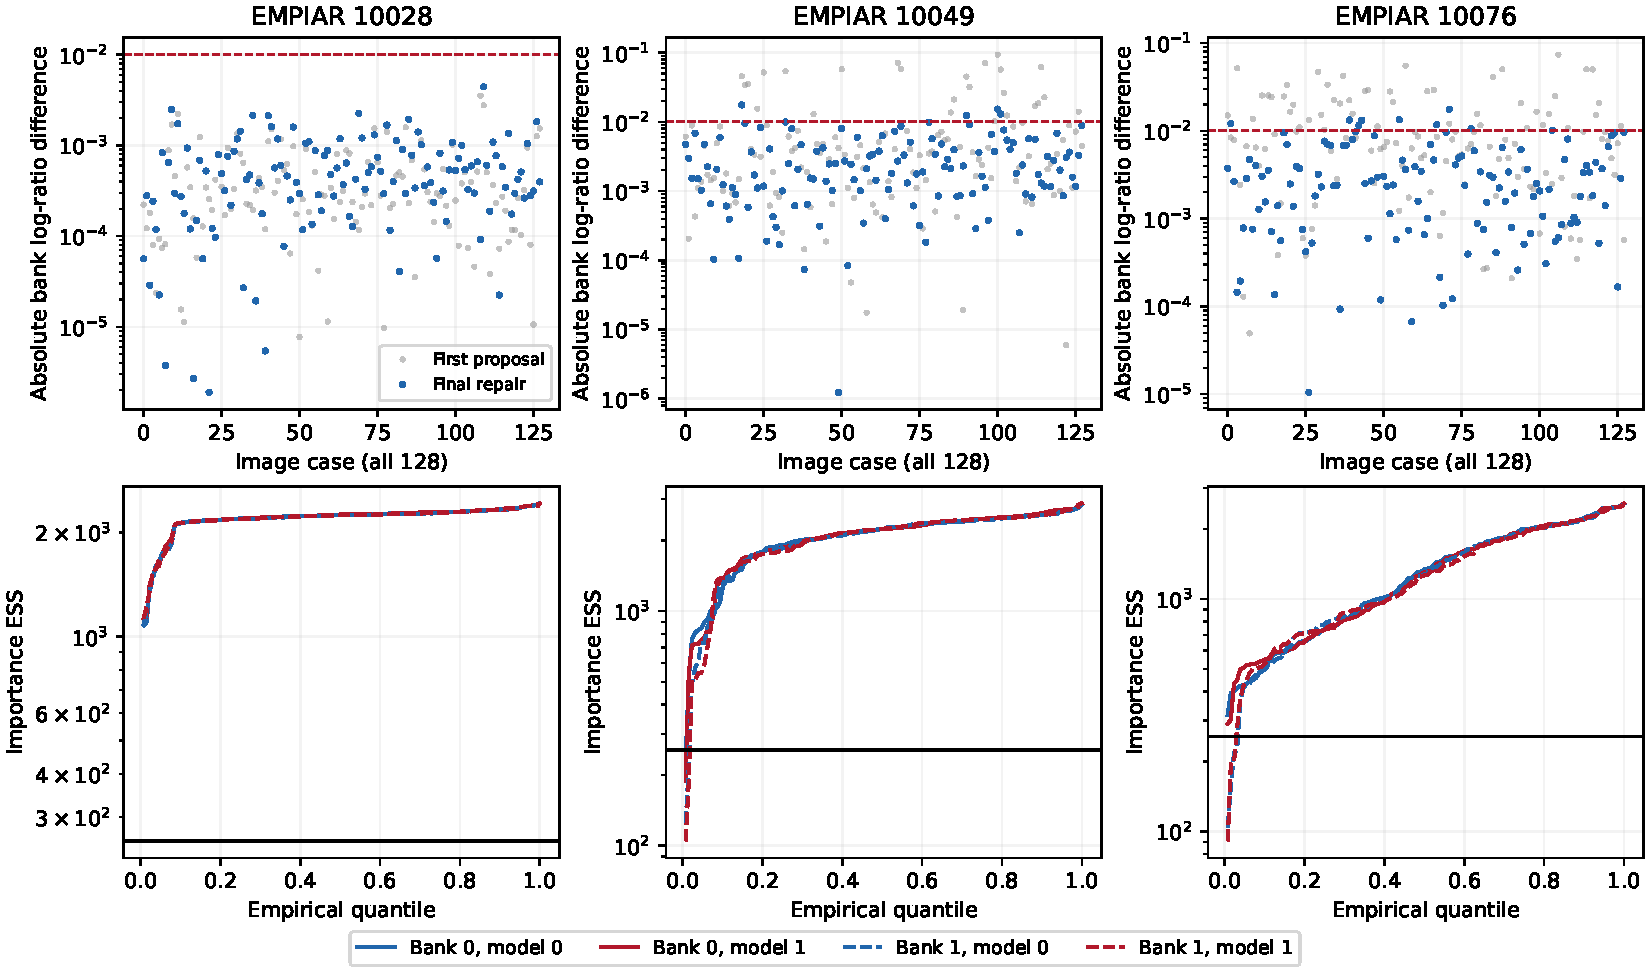
\includegraphics[width=.97\textwidth]{../results/uncertainty/development/catalog-pose-integration-report-v1/final-integration-gate.pdf}
\caption{All 384 image cases of the final integration repair. Top: absolute
bank log-ratio differences, retaining the first proposal in gray and the
repair in blue; the threshold is .01. Bottom: each bank/model ESS distribution,
with the median gate's threshold 256 shown for reference. Thirteen repaired
cases remain outside tolerance. Axis ranges differ by stack. Passing this
necessary numerical gate does not establish an absolute-integral certificate
or experimental uncertainty coverage.}
\label{fig:integration-new}
\end{figure*}

The planted-truth audit retains a failure of the bank-agreement heuristic:
one old 10076 \emph{within-tolerance} case changes by 1.50 log-integral
units after replacing a single draw by truth. After repair, the largest
such jump is .0626. The exact integrals remain unknown. Absolute
log-integral bank RMS after repair is .0288, .0296 and .0424, larger than
ratio RMS .000887, .00452 and .00507. No original local Hessian eigenvalue
was clipped, so covariance clipping does not explain these discrepancies.
The numerical branch ends after this single permitted repair.

\subsection{Recorded nuisances: experimental assumptions remain open}
The full source metadata contain 105,247, 108,544 and 131,899 particles.
For 128 equal-area bins of unoriented plane normals, peak recorded-density
ratios to uniform are 4.53, 6.23 and 2.74; cross-half chi-square summaries
are 1.07, 2.01 and .248. They are inconsistent with treating these recorded
histograms as near-Haar. Estimated poses, symmetries and selection prevent
interpreting them as exact latent distributions or continuous density bounds.
All 90 original histogram vectors independently reproduce.

Four $8\times8$ particle-corner patches per selected particle show nonflat
DCT power, after accounting for Fourier cropping. The relative-coordinate
power ranges are .366--2.101, .783--3.000 and .551--2.162. Particle tails,
small windows and unknown stationarity preclude declaring these pure-noise
spectra. Existing STAR/Frealign joins recover 229, 137 and 351 acquisition
groups for the 8,192-particle cohorts. An earlier missing-group statement
was wrong and is corrected with a complete join/split audit. Between-group
fractions of patch-energy sums of squares are .159, .0724 and .117; these
are descriptive ANOVA fractions, not an intraclass-correlation model.

Per-particle defocus varies substantially, and recorded scale/weight fields
include constants that cannot calibrate physical amplitudes. The alpha--view
association of 2.62\% on 10028 and .74\% on filtered 10076 is a fraction of
recorded alpha variance associated with bins, \emph{not} a percentage
amplitude bound. A single-CTF, known-white-noise simulator remains an
explicit idealization.

\subsection{Population materiality: a scientific failure}
We freeze A as the full fitted map and B as its \emph{full} masked-region
deletion, distinct from the 25\%-deletion discrimination study. All 65,536
saved training rotations are replayed, with direct physical checks at the
first, batch-boundary, halfway and final indices. At $p=.75$, the
known-pose pooled root is evaluated for every prelisted pair: source halves
on all three stacks, and published filtering versus its complement on
10028/10076, each in both state assignments.

These metadata groups are \emph{not biological states}: all three downloaded
class fields are constant zero. Each group's recorded full-rotation
histogram defines a piecewise-Haar proxy on a fixed ZYZ grid. The primary
grid has $8^3$ cells; $4^3$ and $12^3$ are sensitivity analyses. This is
a controlled calculation under proxies, not evidence that two actual
conformations have those laws.

A stack passes only if the same primary pair/assignment has
$|t_\star-.75|\ge .02$ and
$\E_\nu[1/s_\perp]\le8.8125$. The latter gives a nominal local-surrogate
SE .03 at $n=10^4$ after adding $.75\times.25$; it is not an unknown-amplitude
coverage theorem. At least two stacks must pass. No sensitivity grid,
new region or relaxed threshold can rescue a failure.
\begin{table}[t]
\centering\small
\caption{Primary population screen: largest absolute bias and harmonic amplitude-tangent surrogate range across all prelisted assignments. The same pair must meet both criteria; all fail materiality.}
\label{tab:diag-population}
\begin{tabular}{lrrl}
\toprule
EMPIAR & Max. $|t_\star-p|$ & Harmonic range & Gate\\
\midrule
10028 & 0.000214 & 1.291--1.292 & Fail\\
10049 & 0.000122 & 1.039--1.039 & Fail\\
10076 & 0.003493 & 3.872--3.916 & Fail\\
\bottomrule
\end{tabular}
\end{table}

All three fail materiality (Table~\ref{tab:diag-population}); no sensitivity
bias reaches .02 either. Every harmonic surrogate passes, so low modeled
population bias, rather than poor local separation, ends this proposed
method branch. Direct expected-score quadrature independently checks all
30 roots, with residual at most $3.1\times10^{-11}$. Histogram bins and
projected energies reproduce independently. This does not prove general
adequacy of pooled likelihood or impossibility of population inference.

\subsection{Existing population baseline and external controls}
We execute unchanged author functions from \citet{counting2026} on all
23 released two-state likelihood conditions, retaining both successful
and numerically discrepant results. A separate scalar optimizer verifies
the pooled optimum; the weakest synthetic author result differs by .00785,
with small float32 simplex drift. For the published experimental default,
the independent estimate is .798228; under the condition labeled
rotation-10 it is .649749. This is pose-model sensitivity, not a measured
state-view population bias. The .8 experimental reference is a constructed
mixture of classified subsets, not biological truth.

The official CAHRA pose-convention supplement provides 216 high-signal
projections per state. All 432 signed quarter-turn comparisons are retained;
the correct in-plane sign gives median correlation about .988, the opposite
sign about .74. This checks a coordinate convention only. We have not
evaluated the separate noisy 30,000-particle pose/population challenge or
its experimental constructed-mixture task. The requested benchmark access,
noise-only windows and biological state labels remain missing evidence.

\section{Interpretation and Remaining Requirements}
Three distinctions survive these experiments. A low-dimensional summary can
lose discrimination without establishing a limit on the original data.
A numerical integration gate can pass while absolute-integral error remains
too large or insufficiently controlled for inference. A nuisance-robust
population proposal can fail its materiality screen despite plausible local
information. These are separate findings, not interchangeable success claims.

The exact known-pose odds identity diagnoses a specific misspecification;
its extension to latent views and imperfect templates is not supplied.
The amplitude proposition requires nonzero response bias to remain explicit
in bounded-feature constructions. General bias-aware inference, mixture
optimization and deconvolution are established foundations
\citep{donoho1994,armstrong2018,lindsay1983,npmle2024,pensky2017}.
No universal population-coverage theorem or new minimax rate is claimed.

Further method development needs an externally motivated state pair,
a calibrated acquisition/noise model, matched whole-stack population
baselines, repeated unconditional calibration and informative experimental
controls. Repeated fits or model reviews cannot substitute for this evidence.
Four full independent model reviews of earlier drafts rejected the work;
the latest focused consultation motivated the bounded checks here and did
not provide an acceptance verdict. This rewritten diagnostic manuscript has
not received a fifth full review. The work remains an incomplete research
program rather than a demonstrated ICML-level uncertainty method.

\section*{Reproducibility and Impact}
All code, failed attempts, source hashes, numerical arrays and review records
are public at \url{https://github.com/yashpatel5400/fourier-cryo-splats}.
The v0.7.7/v0.7.8 evidence releases and their v0.7.6 dependencies provide the
new experiments; source provenance distinguishes downloaded papers from
executed author code. Gaussian fitting, metadata and conditional simulations
must not be advertised as calibrated biochemical populations. The principal
impact of this work is an auditable account of where the proposed inference
does and does not have support.

\bibliography{references,uncertainty-references,survey-references,diagnostic-references}
\bibliographystyle{icml2026}
\clearpage
\appendix
\section{Proofs and Their Scope}\label{app:proofs-new}
These arguments support the stated diagnostic interpretations. They are not
claimed as a new general framework for inference in mixtures or inverse
problems. In particular, correct algebra conditional on a noise or nuisance
model does not establish that model on experimental particles.

\subsection{Pooled conditional-mixture identity}
For $f_t=t f_A+(1-t)f_B$, write
$u_t=(f_A-f_B)/f_t$. Since $\int(f_A-f_B)=0$,
\begin{align}
\int f_Au_t&=\int\{f_t+(1-t)(f_A-f_B)\}u_t\\
&=(1-t)J_t,\nonumber\\
\int f_Bu_t&=-tJ_t.
\end{align}
Taking expectations over the \emph{state-specific} laws gives
Equation~\eqref{eq:score-new}. An interior zero of that score gives
Equation~\eqref{eq:odds-new}. The second derivative of a conditional
log likelihood is $-u_t^2$, so its expectation is nonpositive, and strictly
negative whenever the conditional components differ with positive probability.
Under the stated strict-concavity condition the zero is the unique interior
optimum. At $t=p$ its score is
$p(1-p)(\E_{\nu_A}J_p-\E_{\nu_B}J_p)$, proving the final statement.
One must evaluate $J$ at the fitted fraction; replacing it by a fixed
discriminability ratio changes this identity into an approximation.

For Gaussian means, let $\ell=\log(f_A/f_B)$ and
$h_t(\ell)=\operatorname{logistic}(\operatorname{logit}(t)+\ell)$.
Then $u_t=(h_t-t)/(t(1-t))$. Subtracting its two conditional expectations,
or using the preceding identities, yields
For $Z\sim N(0,1)$, this gives
\begin{align}\label{eq:gauss-J-new}
J_t(s)&=\frac{\E\{h_t(\ell_+)-h_t(\ell_-)\}}{t(1-t)},\\
\ell_\pm&=\sqrt{s}Z\pm s/2.\nonumber
\end{align}
The implementation integrates the difference before averaging, reducing
cancellation for small $s$. Roots use 64-node Gauss--Hermite quadrature on
$[10^{-7},1-10^{-7}]$ with root tolerance $10^{-10}$; 128 nodes check the
normalized score against $10^{-6}$. A separate verifier integrates the
direct density-ratio score under both generating Gaussians using a distinct
160-node quadrature implementation. None of these checks certifies a
latent-pose marginal likelihood.

\subsection{Harmonic variance and the amplitude tangent}
Conditionally on state $Z\in\{0,1\}$ and pose $R$, the score in
Equation~\eqref{eq:oracle-score-new} is
$Z+\ip{\epsilon}{g(R)}/s(R)$. Its conditional mean is $Z$ and its
conditional variance is $1/s(R)$. Total variance gives
$p(1-p)+\E_\nu[1/s(R)]$; independent images divide that variance by $n$.
No state--view independence is used. The argument requires correct means,
amplitude one, conditional zero-mean unit-covariance noise, $s>0$ and a
finite harmonic moment. It neither proves unbiasedness after noisy pose
estimation nor permits arbitrary view-dependent amplitudes.

At a Gaussian mean with perturbation direction $g$ and real-amplitude
direction $m_A$, the Fisher Gram matrix is
\begin{equation}
\begin{pmatrix}\norm g^2&\operatorname{Re}\ip{g}{m_A}\\
\operatorname{Re}\ip{g}{m_A}&\norm{m_A}^2\end{pmatrix}.
\end{equation}
Its Schur complement is Equation~\eqref{eq:amplitude-new}. This is a
\emph{mean-parameter} calculation, not the efficient information of a
binary mixture with unrestricted amplitude laws. The secondary projection
at $m_B$ is retained in every screen array. Under Haar, projection at the
full map reduces arithmetic mean separation by 4.95\%, 37.14\% and 8.28\%.
The corresponding harmonic surrogates are 1.2912, 1.1206 and 3.9184.
Nonzero local separation is compatible with nonlinear ambiguity or unstable
population inference.

\subsection{Bounded-score amplitude obstruction}
Whiten a nonsingular Gaussian covariance. For bounded measurable $\psi$,
set $F_z(a)=\int\psi(y)\phi_d(y-a m_z)\,dy$. For complex $a=u+iv$,
the modulus of the extended Gaussian integrand is bounded by
\begin{equation}
\norm\psi_\infty\,\phi_d(y-u m_z)
\exp(v^2\norm{m_z}^2/2).
\end{equation}
On compact subsets of $a$, this and the derivatives needed to differentiate
under the integral have integrable Gaussian tails. Hence $F_z$ is entire.
If $F_A=1$ on a nonempty real interval, the identity theorem gives $F_A=1$
everywhere. Likewise $F_B=0$ on its interval implies $F_B=0$ everywhere.
But $F_A(0)=F_B(0)=\E\psi(\epsilon)$, a contradiction.

Zero amplitude is used for analytic continuation, not assumed physically
admissible. A fixed affine combination of finitely many bounded features
is bounded, so the proposition applies to any finite-coefficient calibrated
feature score. It does not supply a quantitative bias--variance lower bound,
rule out nonlinear multi-image estimation or establish a root-$n$ impossibility
result. General linear-functional deconvolution theory is relevant
\citep{pensky2017}, but its detailed rate results have not been verified for
our multivariate, support-constrained model.

\subsection{Reciprocal importance identity and stochastic brackets}
For positive $f$ and $q$, set $w=f/q$, and let $I=\int f$.
Changing the first measure from $f/I$ to $q$ gives
\begin{align}
\E[I_\star^{-1}]&=I^{-1}\E_{q^L}
\left[\frac{Lw(X_1)}{\sum_lw(X_l)}\right]\\
&=I^{-1}.\nonumber
\end{align}
The last step uses exchangeability: the $L$ expectations of
$w(X_j)/\sum_lw(X_l)$ are equal and sum to one. Positivity ensures the
denominator is nonzero. A fixed replacement index is valid; choosing a
replacement according to observed weights is not this experiment.

For a matched joint simulation, generating latent variables conditional on
the observations have the exact posterior law. This familiar identity
underlies bidirectional Monte Carlo \citep{grosse2015}. The proposal may
depend on the image and a fixed independent catalogue, but it must not use
the true pose beyond information already in the image. Other draws must be
conditionally independent of that posterior point. Conditional on an
already fixed generating pose, the posterior-draw interpretation is absent.

For independent images, $\prod_i\widehat I_i$ is unbiased for
$\prod_i I_i$, and $\prod_i I_{\star,i}^{-1}$ is unbiased for its
reciprocal. Markov and a union bound give
\begin{align}
\sum_i\log\widehat I_i-\log(1/\delta_L)&\le\sum_i\log I_i,\\
\sum_i\log I_i&\le\sum_i\log I_{\star,i}+\log(1/\delta_U)
\end{align}
jointly with probability at least $1-\delta_L-\delta_U$. We use
$\delta_L=\delta_U=.025$ for each fixed 64-image state/bank bracket.
There is no simultaneous claim across stacks, states or banks; paired
states share noise and poses and are never multiplied together.
The four final widths per stack range from 7.395--7.398, 7.404--7.415 and
7.508--7.519 log units. The additive floor $2\log40=7.378$ dominates.
These are stochastic simulation brackets, not a practical uniform numerical
certificate for experimental inference.

\subsection{Identifiability is distinct from an unbiased score}
For completeness, consider fixed templates with compact noiseless mean
supports $\mathcal M_0,\mathcal M_1$ generated by a compact nuisance space
and continuous forward map. Allow arbitrary joint state/nuisance laws and
assume measurable probability lifts from each mean support to its nuisance
space. The latter is automatic for a finite catalogue; it is an explicit
assumption here for continuous spaces.

Let $\mu$ be the law of the noiseless observed mean, and add independent
known nonsingular Gaussian noise. Its characteristic function is nowhere
zero, so Gaussian convolution identifies $\mu$ from the infinite-data
observed distribution. The compatible state-1 fractions are exactly
\begin{equation}
\left[\mu(\mathcal M_1\setminus\mathcal M_0),\,
\mu(\mathcal M_1)\right].
\end{equation}
Only state 1 can generate the first set; all state-1 mass lies in the
second. Conversely, assign any desired fraction of intersection mass to
state 1 and lift the resulting measures. Thus disjoint supports identify
the population, despite the bounded-score obstruction above. This is a
classical support/deconvolution argument, not evidence of stable finite-data
recovery or of separation between the actual continuous cryo-EM supports.

An admissible pair of means $a,b$, with whitened distance $d$, gives a
simple finite-sample obstruction. The all-state-0 and all-state-1 Gaussian
experiments have $\mathrm{KL}=nd^2/2$, hence
$\mathrm{TV}\le\min(1,\sqrt n d/2)$. Any interval $C$ covering the
population at level $1-\alpha$ in both experiments satisfies under the
first
\begin{equation}
\Pr(\{0,1\}\subset C)\ge
\max\{0,1-2\alpha-\min(1,\sqrt n d/2)\}.
\end{equation}
Transfer the second coverage event by total variation and use a union
bound. A found, independently checked close pair would be sufficient for
this negative witness; a failed local search would not certify positive
separation. We do not report such a numerical witness in this study.
Density floors or restricted nuisance laws can invalidate point-mass
witnesses and must not be silently discarded.

\section{Numerical Protocol and Independent Checks}\label{app:numerics-new}
\subsection{Proposal density on rotations}
The ACG construction normalizes a four-dimensional Gaussian vector to a
unit quaternion \citep{tyler1987}. For covariance $\Sigma\succ0$, its
density relative to normalized uniform measure on the unit sphere is
$|\Sigma|^{-1/2}(u^\top\Sigma^{-1}u)^{-2}$. It is antipodally symmetric,
so the same normalized density passes to rotations. This expression follows
by integrating the Gaussian radial coordinate; we do not claim a new
distribution or a full audit of Tyler's paper.

For catalogue center $c$ and $s=(8\text{ degrees in radians})/2$, use
$\Sigma_c=s^2I+(1-s^2)cc^\top$. The component density is
\begin{equation}
s^{-3}\{[1-(c^\top u)^2]/s^2+(c^\top u)^2\}^{-2}.
\end{equation}
The local proposal uses eight optimized midpoint modes. Its three-dimensional
Hessian covariance is divided by four in the quaternion tangent coordinates;
the scalar quaternion coordinate has unit variance. The original precision
clamps correspond to .25--30 degree standard deviations. No saved optimum's
eigenvalues actually hit these clamps. Original failed optimizer statuses
are retained, and reused modes are not counted as newly converged fits.

The target maps in the integration experiment are $\rho_0$ and $\rho_{.25}$;
their midpoint is $\rho_{.125}$. Catalogue weights are proportional to
$\exp(\text{midpoint log-kernel}/2)$. Full mixture density is evaluated
over all 32,768 centers in chunks of 256 points. The catalogue broadens
the proposal; the integrand remains a continuous-orientation physical
likelihood. Haar mass .05 provides support and finite variance for these
bounded kernels, but does not ensure useful variance at this draw count.

Each stack uses integer-linspace indices from 0 to 8,191, with 64 indices
and both generating states. Bank seeds are
$261020+\text{dataset}+100\times\text{position}+10\times\text{state}
+\text{bank}$. Both 4,096-point prefixes and 8,192-point endpoints are
retained. The repair changes the sampling algorithm, not selected seeds.
Maps, observations, draw counts and gate thresholds stay fixed.

\subsection{Replay, samples and diagnostic errors}
All saved log integrals, ESS values, maximum weights, ratio differences and
gate decisions are recomputed from kernels and proposal densities. The
independent density implementation uses inverse full $4\times4$
covariances at 32 fixed integer-linspace draws from each bank/image:
8,192 independently checked points per stack. Physical checks explicitly
sum all $64^3$ cells at all 220 frequencies for six selected orientations
per stack, evaluating both maps. These are floating-point consistency checks,
not outward-rounded error certificates or exhaustive direct-sum checks.

For normalized importance weights $w_{lm}$ under model $m$, the plug-in
delta variance for a shared-draw log ratio is
$L/(L-1)\sum_l(w_{l1}-w_{l0})^2$. The between-bank SE combines their
variances. Heavy or missed tails can make this estimate unreliable. We
retain matching-state weight mass on Haar-labeled draws, the source family
of the largest weight, Hessian clipping, and the fixed-index planted jump
for every case. Stratification by the original .01 gate is explicitly
post hoc, not a predictive validation.

\subsection{Rotation regeneration and law proxies}
The population screen regenerates all 65,536 training rotations using seed
$261017+\text{dataset}$. Each batch draws 512 rotations, then the original
$512\times220$ real and imaginary noise arrays. Skipping those intervening
draws would produce different later rotations. Direct cell checks at
indices 0, 511, 512, 32,767, 32,768 and 65,535 verify both full and region
means; maximum discrepancy is $1.08\times10^{-11}$.

Full-rotation bins use intrinsic ZYZ coordinates
$\alpha/(2\pi),(\cos\beta+1)/2,\gamma/(2\pi)$, with periodic angular
wrapping. Equal-width cells have equal Haar volume. For metadata mass $p_c$
and $n_c$ training rotations in cell $c$, each such rotation receives weight
$p_c/n_c$. An occupied metadata cell with no training draw would make that
grid unavailable; no such case occurred. The independent verifier derives
Euler angles from rotation-matrix entries and reconstructs every histogram.
These finite histograms define the tested proxies. They are not an estimate
with guaranteed error against the true continuous state-specific viewing law.

\section{Sampling Errors and Complete Outcome Scope}\label{app:stats-new}
Let $x_i=T_{0i}$, $h_i=T_{1i}-T_{0i}$, $\widehat\mu=\bar h$ and
$\widehat v=(n-1)^{-1}\sum_i(x_i-\bar x)^2$. A delta influence for
$\widehat D=\widehat\mu^2/\widehat v$ is
\begin{align}
\widehat\varphi_i={}&\frac{2\widehat\mu}{\widehat v}(h_i-\widehat\mu)\\
&-\frac{\widehat\mu^2}{\widehat v^2}
\left\{\frac n{n-1}(x_i-\bar x)^2-\widehat v\right\}.\nonumber
\end{align}
We report $\operatorname{sd}(\widehat\varphi_i)/\sqrt n$ as an
asymptotic conditional Monte Carlo SE. It includes gap/variance covariance;
the SE of the gap alone is not an SE of $D$. Three empirical-contamination
finite differences verify this influence for every one of 96 entries.
No finite-sample confidence bound or power guarantee is attached to it.

Population-law linear summaries report within-cell Monte Carlo SEs
conditional on fixed bin counts: if $v_c$ is the sample within-cell
variance, the estimated variance is $\sum_cp_c^2v_c/n_c$.
This does not include pose, template, histogram-estimation or noise-model
error. The exact root is checked numerically, not assigned an experimental
confidence interval. Both assignments of each law pair and all three grids
are retained; no outcome-guided subgroup or cell selection is performed.

The study's accounting units are important. There are 384 integration image
cases, formed from 192 source images across three stacks and two paired
states; the paired states are not independent source particles. Each attempt
has two banks per case. There are 30 population pair/assignment/grid
comparisons, not 30 independent biological experiments. The template-score
ledger has 96 rows sharing images, models and banks. Method comparisons use
shared draws intentionally; row counts must not be treated as replication
counts for statistical significance.

\section{Critical Survey and Unresolved Scientific Questions}
\label{app:survey-new}
The living survey is dated 1 October 2026. It contains 141 curated
bibliographic candidates and a much larger broad-search ledger that is not
an individually read methods corpus. Source manifests record versions,
access failures and reading depth. We distinguish published papers from
versioned preprints, targeted full-text reading from abstract screening,
and original-code execution from descriptions of published experiments.
This is a substantial scoped survey, not a claim of exhaustive field coverage.

\paragraph{Density posteriors and model error.}
RELION's Bayesian formulation, Gaussian pseudo-atom inference and
probabilistic Fourier-slice models are direct uncertainty antecedents
\citep{scheres2012,joubert2015,ullrich2020}. Their posterior assumptions
should not be erased by calling them deterministic baselines. Likelihood
Hessian tails expose weak density--pose directions \citep{rangan2024}.
Dynamic empirical-Bayes/MCMC approaches also study confidence and resampling
targets \citep{lai2023}. An additional posterior ensemble is therefore not
novel merely because its representation is Gaussian. Meaningful comparison
requires equal nuisance assumptions, information and scale, including a
matched prior baseline where appropriate.

\paragraph{Pose distributions and confidence statements.}
Posterior-averaged rotations \citep{bayespose2026} and probabilistic search
in SIMPLE \citep{simple2025} address estimation. Cryo-forum's dispersion
supports ranking and filtering \citep{cryoforum2023}. CESPED explicitly
uses refinement-derived experimental labels with their own uncertainty
\citep{cesped2024}; ARCHER and cryoPARES investigate transfer and pose
prediction \citep{archer2026,cryopares2026}. Their scores cannot be
substituted for a uniformly valid per-particle error radius without checking
the guarantee and deployment relationship. The recent Bayesian orientation
paper's Appendix F discusses joint prior estimation and sensitivity;
simply fitting a preferred-view prior is already an explicit direction.

\paragraph{Heterogeneity representations.}
CryoDRGN, DynaMight and 3DFlex describe different density or motion families
\citep{zhong2021,dynamight2024,flex2023}. RECOVAR uses covariance estimation
and kernel regression \citep{recovar2025}. Physical heterogeneity is a
distribution of molecular states, not automatically posterior uncertainty
about a single mean density. Independent-half deformation disagreements
and held-out motion validation have specific targets; shared learned
components and evaluated frequency bands matter. Gaussian GMMs, CryoSplat,
GEM and hierarchical parts are substantial representation prior art
\citep{chen2021,chen2025,qu2025,shekar2025}. Fourier conjugate pairing differs
from real-space splats, but needs demonstrated value beyond that distinction.

\paragraph{Population and thermodynamic uncertainty.}
Cryo-BIFE integrates image nuisances and samples free-energy profiles on a
fixed path \citep{cryobife2021}. Our follow-up reads the main synthetic
sections, all seven supplement pages and all six supplemental figures;
we do not execute its MCMC. Its controls vary noise, defocus, count and path,
and include posterior-versus-MAP/assignment comparisons. A visible reference
outside an interval in one realization is not a frequentist coverage study.
The method's nuisance integration must not be replaced by a weak known-pose
baseline when comparing future work.

Whole-stack population inversion and classification counts can differ
substantially \citep{counting2026}; our 23-condition author-code replay
supports that computational distinction using supplied likelihoods.
Measurement-limited ensemble granularity \citep{mattingly2026} and
discretization error \citep{mordant2026} directly constrain claims about
resolvable populations. cryoTWIN targets thermodynamic landscapes
\citep{cryotwin2026}. Targeted SI-3/SI-4 reading finds training-subset/seed
and fixed-landscape path variability measures, rather than repeated-sampling
coverage. Its comparisons include resolution and density-construction
differences that require matching in our own studies. We did not audit
all its proofs, figures or code.

\paragraph{Population uncertainty versus selection.}
Even accurately estimating the fraction among retained images does not
recover solution-state populations without assumptions about particle
capture, picking, classification and filtering. Constructed mixtures
provide controlled source proportions but not complete molecular density
truth. Selection and pose-model sensitivity must not be conflated with
state--view dependence. The author-released rotation-10 result in our replay
demonstrates sensitivity to a changed likelihood input, not its causal
attribution to a biological viewing law.

\paragraph{Moment and distributional methods.}
Nonuniform moment reconstruction, compressed moment recovery and
moment-based candidate comparison already estimate or profile viewing laws
\citep{sharon2020,subspacemom2026,momentmetrics2024}. Their bandlimit,
genericity, identifiability and acquisition assumptions matter. High-noise
likelihood theory \citep{fan2024} does not calibrate individual poses.
Recent moment-conditioned posterior sampling and functional deconvolution
study distinct compressed-information models
\citep{janson2026mps,alghattas2026functional}; their full code and proofs
were not replicated here. Distributional inverse stability
\citep{stochastic2026} further distinguishes image-distribution fit from
latent reconstruction error under explicit stability assumptions.
The failure of our low-order scores cannot rule out collective recovery.

\paragraph{Map validation and learned priors.}
Independent halves, noise substitution, directional resolution and
independent-particle validation have complementary roles
\citep{schereschen2012,chen2013,monodir2020,independent2020}.
FDR confidence maps test density significance \citep{beckers2019,beckers2020}.
Blush regularizes reconstruction using learned information
\citep{blush2024}; LocScale-2.0 attaches confidence to map enhancement
against its specified proxy \citep{locscale2026}. Bias/variance discussions
already explain why consensus is insufficient \citep{sorzano2022}.
Sharper appearance, half-map agreement and enhancement confidence do not
share one calibration claim, and cannot be ranked by an inappropriate
single coverage metric.

\paragraph{Atomic and multimodal targets.}
EMMIVox combines molecular information with map-based likelihoods
\citep{emmivox2024}; experiment-guided AlphaFold3 addresses structural
ensembles with multiple measurement types \citep{guidedaf32026}.
CalPro's coordinate-error target uses a different calibration unit
\citep{calpro2026}. An atomic-model score is neither a raw-particle density
interval nor a population confidence bound. Independent modalities can
test interpretations that an image model alone leaves ambiguous.

\paragraph{Conformal and simultaneous calibration.}
Posterior-variance calibration and quantile/conformal inverse imaging rely
on a specified population of signal--observation pairs
\citep{narnhofer2024,qutcc2026}. Noise draws or neighboring voxels from one
molecule are not automatically exchangeable new molecules. Simultaneous
inverse confidence regions \citep{batlle2025} differ from many separately
calibrated marginal intervals. Bias-aware optimal recovery and GP/ridge
connections are also established \citep{donoho1994,armstrong2018,kanagawa2025}.
A conditional theorem, an empirical error ranking and marginal population
coverage require different evidence.

\paragraph{Gaussian uncertainty beyond cryo-EM.}
Bayesian splatting, photometric uncertainty, view-structured conformal
prediction and radiative CT consider different forward models and targets
\citep{jia2026bayesiangs,galappaththige2026ppu,chu2026viewcp,zhao2026radiative}.
Their existence further limits a claim based only on attaching variance
to Gaussian kernels. Translating a method requires checking the change from
view synthesis or CT measurements to latent-pose Fourier projections, and
from prediction error to structural or population inference.

\paragraph{Benchmark construction and remaining access.}
CAHRA version 2 describes three separate challenges
\citep{cahra2026}: experimental compositional mixtures, simulated
conformational variation, and pose/population entanglement. The last uses
two CALHM2 structures with preferred views and Gaussian noise, sampling
state and view independently. A 3\% uniform component is a density
\emph{floor}, not an upper bound on peak viewing density. Public benchmark
proportions are known, so subsequent use is not a blind challenge entry.
The separate convention supplement has been downloaded and checked here;
the main 8\,GB pose benchmark remains behind a Globus sign-in requirement.
Its live leaderboard is not a substitute for a methodological comparison
with identified baselines and uncertainty metrics. Challenge-1 frame overlap
and common preprocessing must be checked before treating frame sums as
independent measurements.

\paragraph{Open questions supported by this survey.}
The strongest unresolved questions are population uncertainty under template
and viewing-law error; calibrated absolute pose confidence; validation of
detail introduced by learned priors; and propagation through CTF estimation,
preprocessing, alignment and molecular interpretation. These are conclusions
about priorities, not claims that no relevant prior work exists. For this
project, a real source-labeled mixture and a defensible noise model are more
valuable than another minor variant of the failed compact-region method.

\section{Historical Comparisons and Reproduction}
\label{app:repro-new}
The original reconstruction and uncertainty studies are not erased by this
rewrite. Their PDFs, source snapshots and exact outcomes remain in tagged
releases. The new manuscript reorganizes the scientific question; it does
not convert old conditional results into experimental calibration.

\paragraph{Reconstruction baselines.}
Three 8,192-particle datasets have Gaussian, trilinear and stock homogeneous
neural fits using public consensus poses. The Gaussian/voxel test NMSE pairs
are .83313/.83939, .93023/.93103 and .87503/.87909. These are normalized
image prediction errors in the original preprocessing, not population error.
Conditional half-map FSC remains above its threshold at the sampled limit,
so nominal resolutions 16.08, 7.872 and 13.973\,\AA\ are censored limits,
not independently resolved atomic detail. Backprojection is named separately
from neural training. Unknown-pose RELION finishes on all three stacks with
its convergence and registered-reference diagnostics retained. No ab initio
CryoDRGN-AI result is substituted for those distinct experiments.

\paragraph{Density-interval failures.}
The earlier continuous audit compared a finite fitting dictionary with a
larger supported density class. A matched continuous Gaussian-prior
comparator shares its fixed-pose guarantee at the stated scale, so coverage
was not an advantage over that baseline. The complete matched rerun has
48 converged fits and 672 conditional cases. A separate local-refinement
study has 600 simulated datasets and 12,000 weight fits; all 216 reported
procedure/control cells cover broad targets in 200/200 trials, but all three
pose-audit procedures select the no-data fallback. Raw median widths are
642--1,242 times that fallback's width. A local optimizer worsens the
near-truth initialization; it is not a production-refinement comparison.
Noise-only coverage of one pilot-aligned 10049 feature is .720 versus .955
with true poses in the saved-draw replay. These findings motivate caution
about plug-in alignment but do not prove a collective cryo-EM limit.

\paragraph{Moment methods and closed development.}
Power/bispectrum variants, classical concentration comparators, covariance-
aware contrasts and equal-noise-budget allocations remain in the prior
evidence releases. Their scope is controlled candidate validation, not
population coverage. The new matched ledger and metadata audit address
the information and nuisance questions those studies left open. No new
moment variant is selected in this manuscript. The historical allocation
text contained a transcription .000182; its source result is approximately
.0001755. This does not affect the new matched comparison or gate outcomes.

\paragraph{Author-code population replay.}
The upstream commit is \texttt{b9099e1b7fb3}; the full identifier is retained
in the replay manifest.
Its original likelihoods are reused, not regenerated. All 10 synthetic and
13 experimental conditions are retained; two separately named noisy-image
inputs are byte-identical and are not independent controls. The synthetic
empirical label fraction .80074 differs from generator probability .8.
The original float32 weights deviate from sum one by up to
$1.82\times10^{-5}$; raw and normalized diagnostics remain visible.
The replay uses current isolated dependencies, not an exact reproduction
of the authors' environment. It executes their functions without copying
their implementation into our package.

\paragraph{Executable provenance.}
Separate runners, verifiers and reporters implement catalogue integration,
population materiality, the saved-draw integration autopsy and fixed-bank
separation. Exact script names and commands are in the repository's
\href{https://github.com/yashpatel5400/fourier-cryo-splats/blob/uncertainty-study/research/uncertainty/REPRODUCE-POST-REVIEW4-GATES.md}{post-review reproduction document}.
Archive manifests enumerate source commits, input hashes, byte lengths and
dependencies. Replays refuse to overwrite their original records; a new
audit needs a separately named output. We retain failed dependency/packaging
attempts and correct their provenance rather than deleting them.

\paragraph{Independent review and resource use.}
The exact external model was \texttt{claude-fable-5-1}; four full earlier
reviews reject at confidence 4/5. The post-round-4 methods consultation
read supplied text, did not execute arrays or browse papers, and suggested
the bounded population screen. Its unchanged visible response, prompt and
provider identity are preserved; private reasoning is excluded. The
catalogue repair was frozen and started before its critique was retrieved,
although the provider had completed it shortly earlier. The actual .45 local
mass does not follow its later local-majority suggestion. No parameters were
changed to produce a favorable result. A model's approval would not establish
conference acceptance, and no fifth full review has been requested for this
diagnostic rewrite. All current work uses the Mac; no GPU rental is needed
for the completed diagnostics.

\end{document}
